\subsection[Architektura]{Architektura}
\begin{figure}[H]
    \centering
    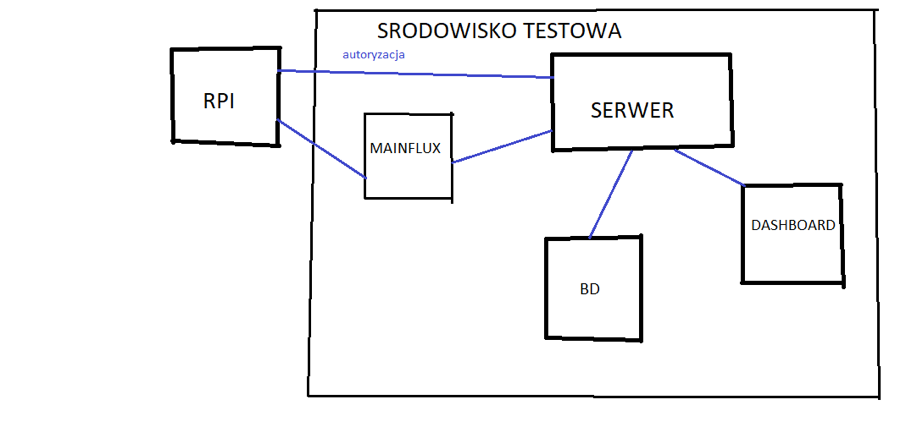
\includegraphics[width=\textwidth]{kp01}
    \caption{Placeholder}
    \label{fig:iotarch}
\end{figure}
\begin{itemize}
    \item SERWER - //jak działa jak jest podzielony //diagram klas dla serwera?
    \item MAINFLUX - //bardzo ogólnie
    \item BD - //również ogólnie //co kiedy się zapisuje?  //pyt czy powiedzieć czemu taką bazę 
    \item DASHBOARD - 
    \item RPI – //co potrzebuje do połączenia się z serwerem // czy dodać coś o bd na rpi?

\end{itemize}

 


